% !TEX root = main.tex

\section{进程}
\subsection{基本概念}
进程(process)是\textbf{运行时(running/in execution)}程序的实例。
\begin{itemize}
	\item 程序并发执行的特征(多道程序):间断性、无封闭性、不可再现性(破环冯顺序执行特性)
	\item 进程的特点:动态性、并发性、独立性、异步性
	\item 进程的作用
	\begin{itemize}
		\item 提升CPU利用率:将多个进程重叠(一个进程IO时另一个计算)
		\item 降低延迟(latency):并发执行,不断切换,防止卡住
	\end{itemize}
\end{itemize}

进程控制块(Process Control Block, PCB),在Unix是\verb'proc',在Linux是\verb'task_struct'
\begin{itemize}
	\item 进程标识符/ID
	\item 进程状态:运行、就绪、等待/阻塞、创建、结束、挂起等
	\item 优先级
	\item 程序计数器(PC)
	\item 内存指针:报错指向程序代码、相关数据和共享内存的指针
	\item 上下文数据(context):进程被中断时寄存器中的数据
	\item IO状态信息
	\item 记账信息(accounting):占用处理器时间、时钟数总和、时间限制等
	\item 链表:各状态的进程形成不同的链表:就绪链表、阻塞链表等
\end{itemize}

进程映像:\underline{进程控制块PCB}(用于进程控制于调度)、\underline{程序段和相关数据段}(用于运行程序)、\underline{系统栈}(跟踪过程调用及参数传递)、\underline{共享地址空间}(进程间通信)。

\subsection{进程状态模型}
多状态进程模型如下,其中挂起进程指进程\textbf{映像}在外存中等待被调入内存(又分为六状态和七状态模型)。
进程由运行态转入阻塞态的原因是\underline{I/O中断、系统调用},这是一个主动的过程。
而由阻塞态转入就绪态则是被动的过程。
\begin{figure}[H]
	\centering
	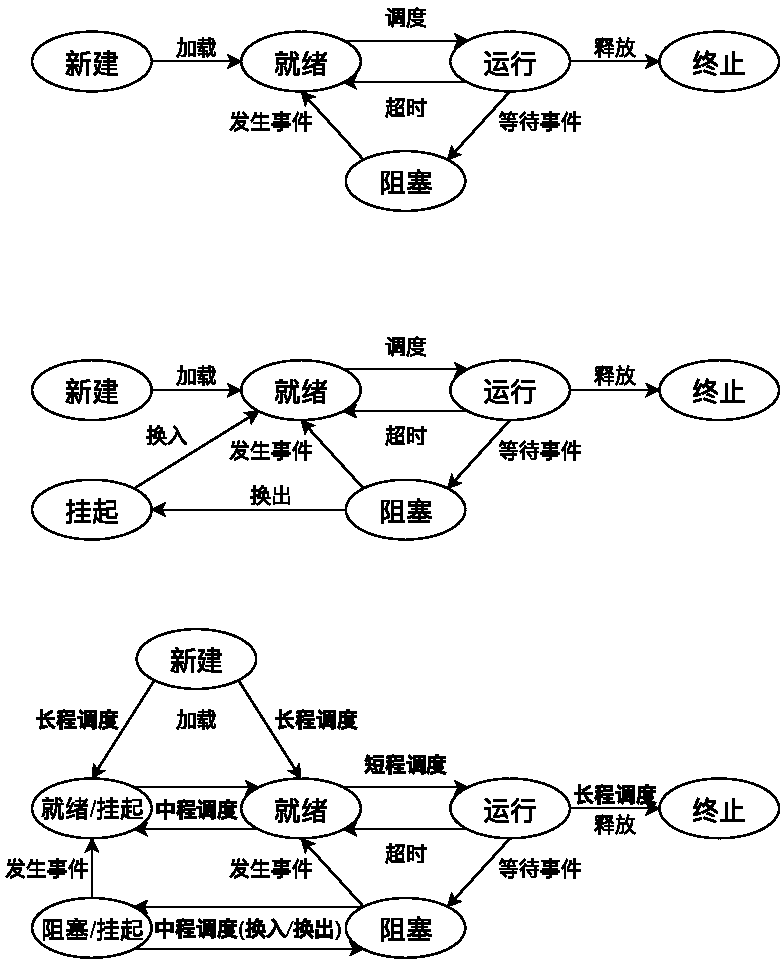
\includegraphics[width=0.6\linewidth]{fig/OS.pdf}
\end{figure}

\subsection{进程的操作}
进程的创建
\begin{enumerate}
	\item 分配唯一的进程ID
	\item 分配进程所需的资源:内存空间(页面)、栈
	\item 初始化PCB:ID、状态、优先级等
	\item 如果可以则加入就绪队列(长程调度)
\end{enumerate}

% 如果想要进程之间交互,则通过文件进行,如sublime编辑文件,gcc对其进行编译
进程间的通信
\begin{itemize}
	\item 共享存储:进程到共享空间再到进程
	\item 消息传递:直接进程到进程
	\item 管道通信:进程到缓冲区到进程,管道即共享文件,半双工通信
\end{itemize}

进程控制由原语(primitive)完成,由若干条指令完成,也可被视为原子操作

内存组织:代码段、数据段、堆段、栈段(从小地址往大地址)
\begin{figure}[H]
\centering
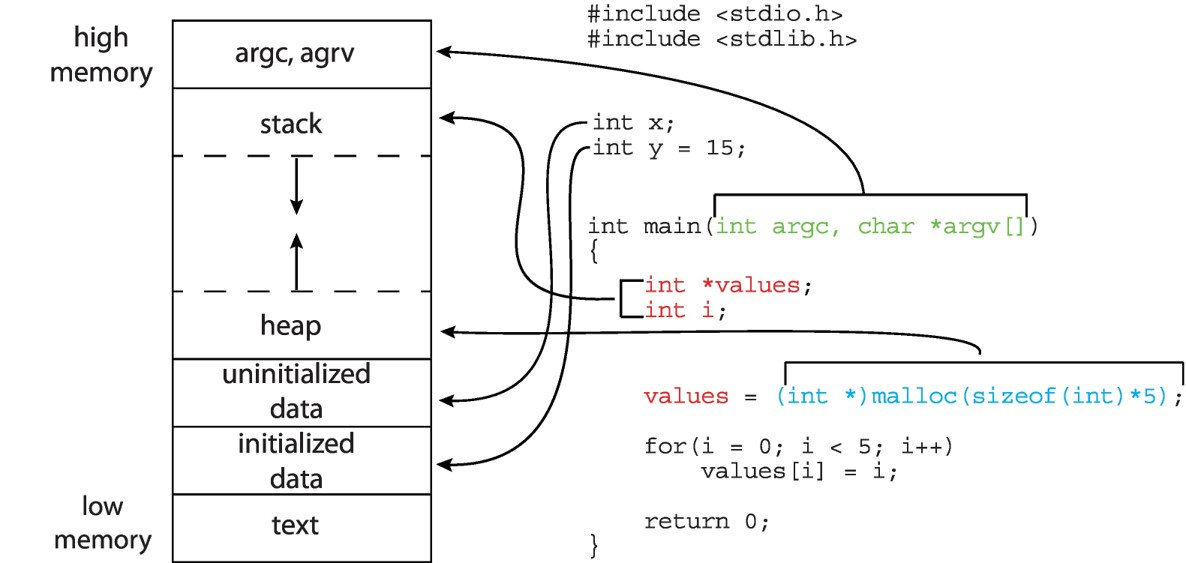
\includegraphics[width=0.8\linewidth]{fig/C_memory.jpg}
\end{figure}

可以参考原始的UNIX论文\footnote{\url{http://www.scs.stanford.edu/19wi-cs140/sched/readings/unix.pdf}}。
\begin{itemize}
	\item 创建进程:fork、waitpid
	\item 删除进程:exit、kill
	\item 执行进程:execve
\end{itemize}

% COM 基于组件共享技术 软件重用
% OLE

导致OS获得控制权的事件:
\begin{itemize}
	\item 时钟中断:时间片结束
	\item IO中断:IO完成
	\item 硬件中断/陷阱(trap)/异常
	\item 系统调用:\verb'int'
\end{itemize}

\par ​​​​​​​可重入性(reentrant)函数:可以被一个以上的任务调用,而不必担心数据的破坏。可重入型函数任何时候都可以被中断,一段时间以后又可以运行,而相应数据不会丢失。可重入型函数或者只使用局部变量,即变量保存在CPU寄存器中或堆栈中。如果使用全局变量,则要对全局变量予以保护。
如\verb'strcpy'是可重入的,而\verb'swap'是不可重入的。
% https://blog.csdn.net/sinat_39440759/article/details/86695230

可再入式内核:一个进程中断后,内核会保存当前进程的相关信息,然后执行下一个进程,等完成后再将上个进程从中断的位置重新恢复执行。
Linux内核是可再入的,这意味着几个进程可能同时在内核模式下执行。(当然单处理器系统,在某一时间只会有一个进程执行,但许多会阻塞在内核模式)这些进程会分时共享CPU、I/O设备等系统资源,给用户的感觉就像是在同时运行。